\documentclass[./dokumentation.tex]{subfiles}

\begin{document}
\chapter{Emotionen - Grundlagen}
Nach  \cite{vanGorp2013} können Emotionen anhand von zwei grundlegenden Dimensionen beschrieben werden. Diese Dimensionen sind Wert (Value) und Erregung (Arousal). Den Wert von etwas bestimmen wir irgendwo zwischen Gut und Böse, was häufig mit angenehm oder unangenehm verknüpft wird. \\
Bei Erregung handelt es sich um die unbewusste Aktivierung des Körpers, Gehirns oder eines bestimmten Verhaltens. Dieses wird durch das Ausmaß von Angst gegenüber Schläfrigkeit definiert und kann beispielsweise durch das Überwachen von Herzfrequenz, Atmung oder Blutdruck gemessen werden. Werden beide Emotionsdimensionen, also das Bewusste, Kognitive und das Unbewusste, Körperliche kombiniert, erhält man das kreisförmige Emotionsmodell, welches in ähnlicher Form schon 1980 von Russell aufgestellt wurde.\\ 
Dieses ist in der folgenden Darstellung (\ref{fig4:affect}) abgebildet und enthält noch zusätzlich Affekte, wie Zufriedenheit (Contentment), Aufregung (Excitement), Not, Verzweiflung (Distress) und Niedergeschlagenheit (Depression), welche jeweils zwischen den Achsen eingeordnet werden können  (\cite{Russell1980}). \\

\begin{figure}[H]
    \centering
    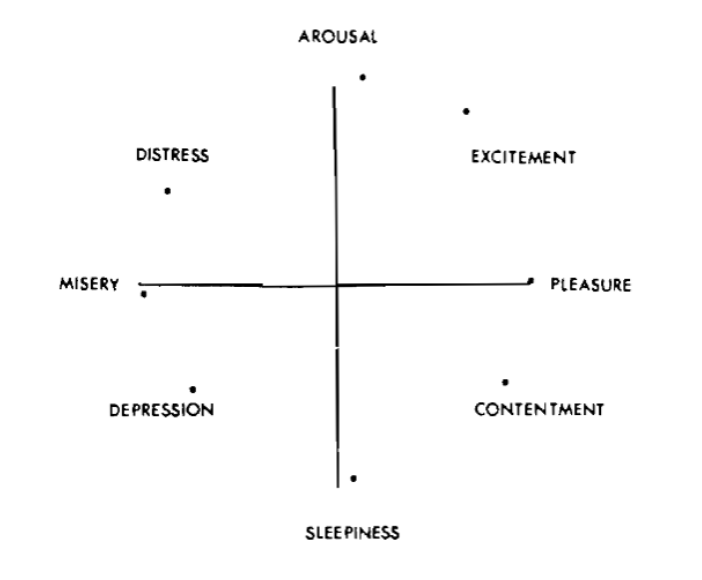
\includegraphics[width=0.8\textwidth]{bilder/russell1.png}
    \caption{Acht Affektkonzepte in kreisförmiger Ordnung (\cite{Russell1980})}
    \label{fig4:affect}
\end{figure}\\

Analog dazu können auch weitere Affekte in den Kreis eingeordnet werden. In der folgenden Abbildung (\ref{fig5:28affect}) nach Russell sind 28 Affekte innerhalb des Kreises dargestellt.

\begin{figure}[H]
    \centering
    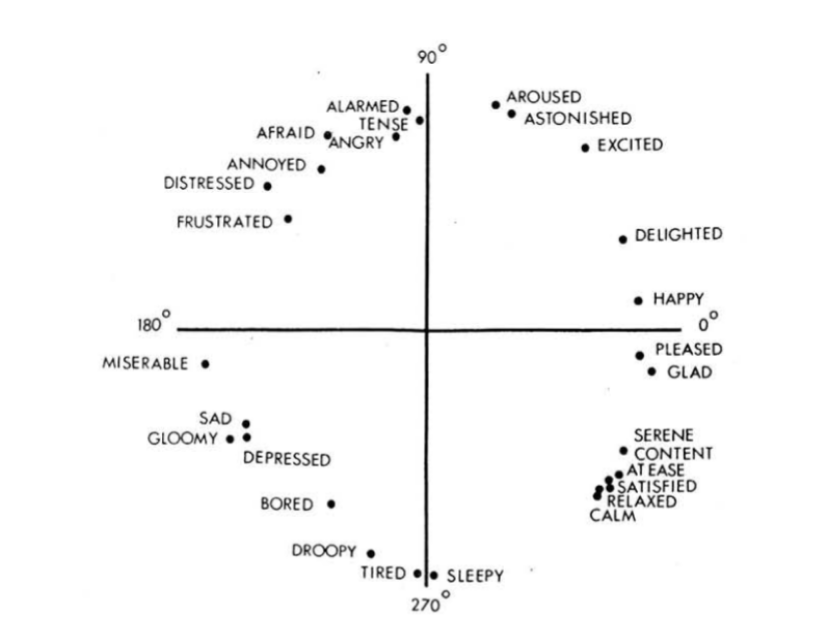
\includegraphics[width=0.8\textwidth]{bilder/russell2.png}
    \caption{Direkte kreisförmige Skalierungskoordinaten für 28 Affektwörter (\cite{Russell1980})}
    \label{fig5:28affect}
\end{figure}\\


\end{document}


